%----------------------------------------------------
\section{The OpenETCS tool chain}
%----------------------------------------------------
\subsection{Definition}
%----------------------------------------------------
The tool chain provides the tool support and the development process
to provide a formalized specification of \gls{SRS} and an executable
code of the \gls{OBU}.


The tool chain is composed by two kind of tools :
\begin{enumerate}
\item {\it Development tools}: those used along the phases of the software
  development process (Requirement engineering, modeling ...).
\item {\it Management tools}:  those used transversely during the
  complete development process (version management, requirements
  traceability ...).
\end{enumerate}
These tools are called vertical and horizontal tools in
\cite{wasserman_tool_1990}. 
Figure \ref{fig:toolchain} shows the idea of the complete tool chain
integration.

\begin{figure}[htbp]
\centering
  \includegraphics[width=.5\textwidth]{images/toolchain_archi-dev}
  \caption{The OpenETCS tool chain}
  \label{fig:toolchain}
\end{figure}

In the next chapters  we will give more details on the
data integration between the development tools by defining the inputs
and outputs artifact of each tools. This document describes the
interface between the tool chain activities.
The interoperability mechanism will be defined in a separate
document. However, the first version of the tool chain will implement a
file-based data exchange.
 
It has been decided (see \cite{D7.1}) that the tool platform hosting
the tool chain is Eclipse with the Eclipse modeling framework
(\gls{EMF}).  This implies that the tool chain will be a set of
Eclipse plug-ins. It also implies that we can rely on already
available plug-in and features for the versioning, the project
management or the build system.  The use of EMF will also assist the
software development, by providing a meta model and an \gls{API} for
manipulating EMF components.


%----------------------------------------------------
\subsection{The SysML Model}
%----------------------------------------------------
A SysML model of the tool shown figure \ref{fig:overview} . It
allows us to have a formal representation of the tool chain and
help to model precisely the different interaction between the
development tools as well as the management tools.  The SysML model
may be also seen as a guideline for integrated new tool: each new tool
should be fully described and comply to the defined interfaces.
Moreover following the idea of Slotosch \cite{slotosch_iso_2012} the
model will be the basis to the qualification analysis \cite{D7.3}.

\begin{figure}[htbp]
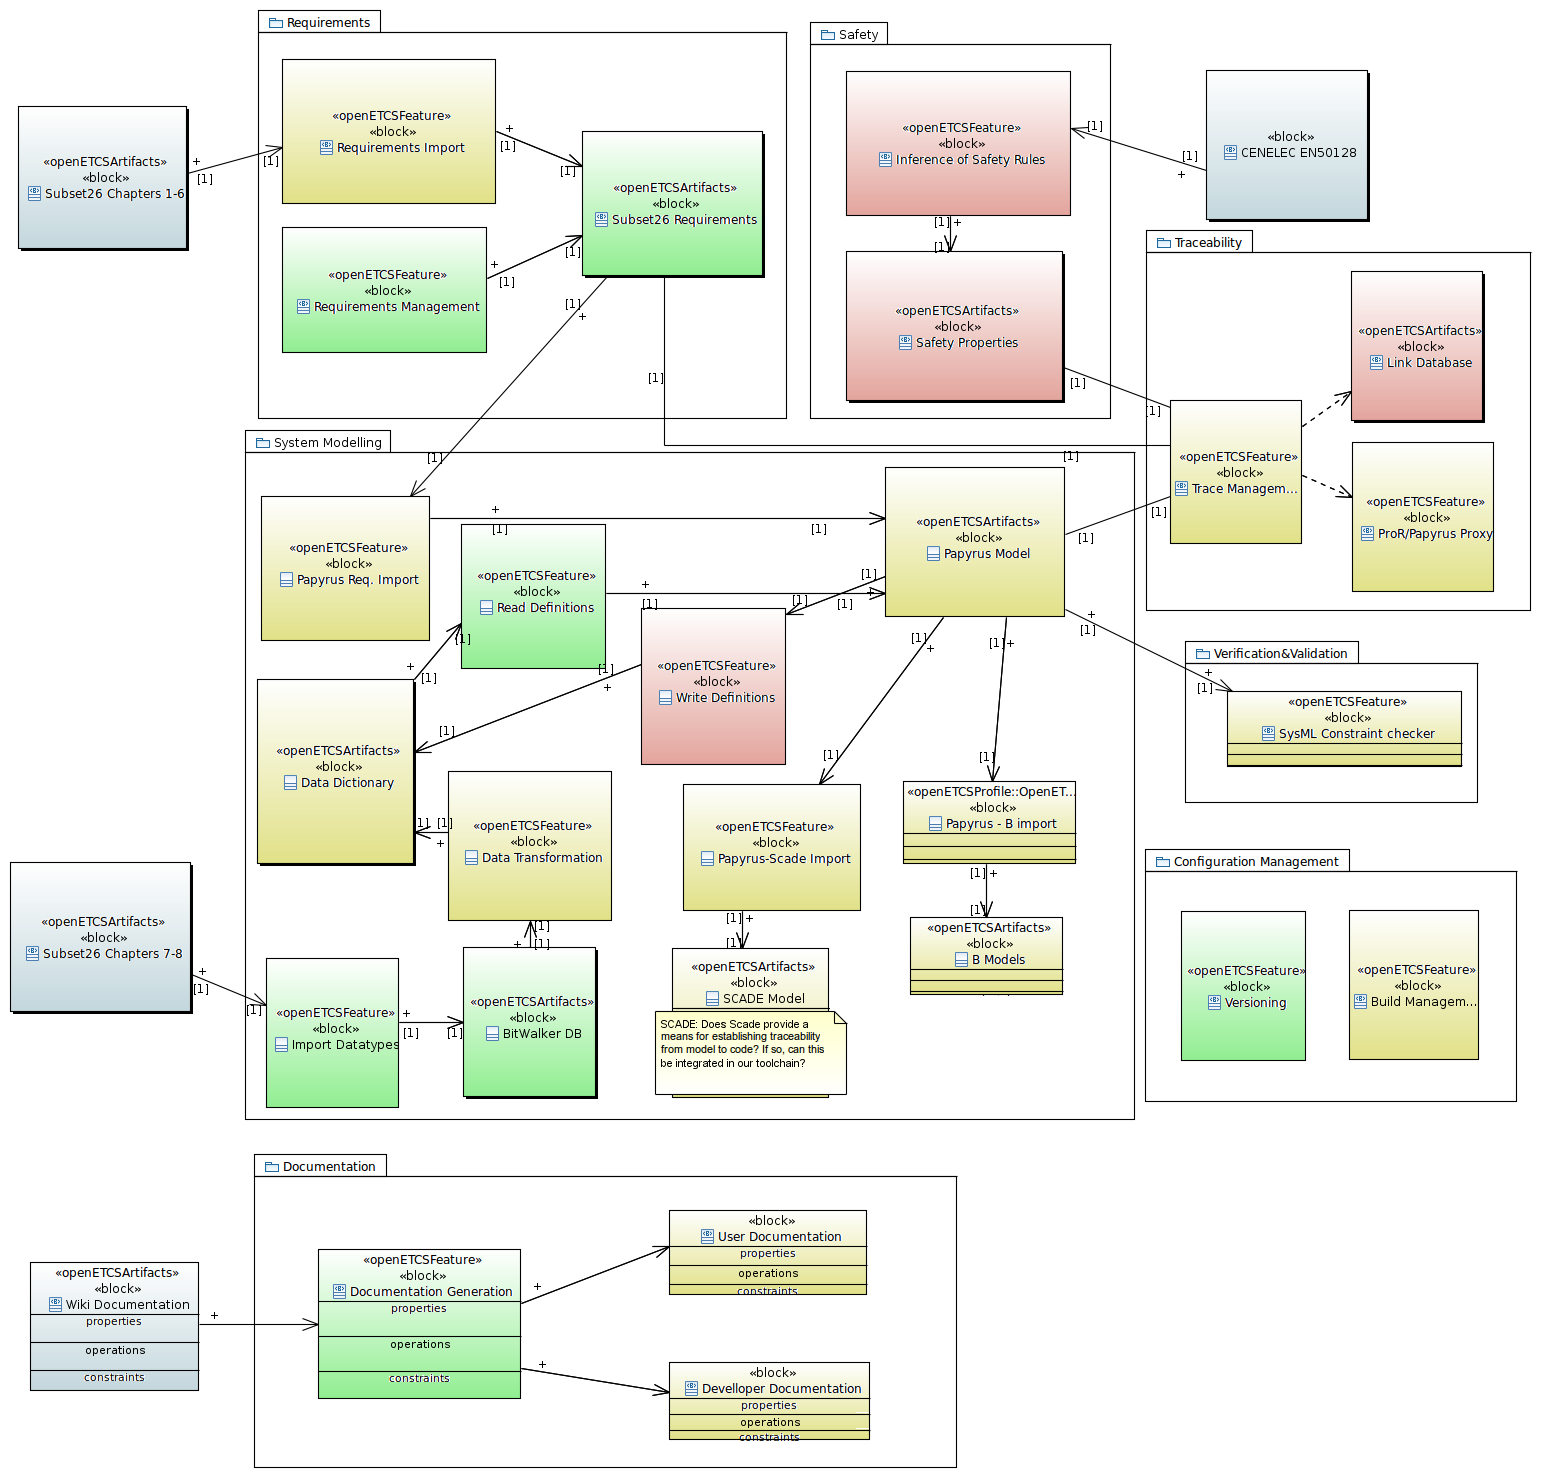
\includegraphics[width= \textwidth]{images/ToolChainmodel.png}
\caption{\label{fig:overview}OpenETCS tool chain Status Overview}
\end{figure}
\todo[inline]{Check if the overview is up-to-date and complient with
  the real implementation}

The requirements of WP2 \cite{baro_requirements_2013} as well as our
intern requirements (Appendixes \ref{app:wp2req} and \ref{app:WP7Req})
will be included in the SysML model. Each tools and their connections
should then also comply to the requirements list.


%----------------------------------------------------
\subsection{The OpenETCS lifecycle}
%----------------------------------------------------
\todo[inline]{Insert the tool chain lifecycle definition from WP1}
%----------------------------------------------------
\section{OpenETCS \gls{EVC} lifecycle}
%----------------------------------------------------
The openETCS lifecycle has been defined in 
 \cite{D2.3} as  presented figure \ref{fig:openETCSProcess}.
\begin{figure}[htbp]
  \centering
  \includegraphics[width= \textwidth]{images/ProcessOpenETCS}
  \caption{openETCS Process (rough view)}
  \label{fig:openETCSProcess}
\end{figure}

The lifecycle defined all the different steps needed to produce a
\gls{EVC} certifiable SIL4. However in order to define a tool chain we
need to define the lifecycle by means of activities
(Fig. \ref{fig:openETCSActivities}). Each activities may be achieved by
one or more tools in the tool chain. 

The next chapters will define the limits of each activities, we will
show what should be consumed and produced by each activities. 
\begin{figure}[htbp]
  \centering
  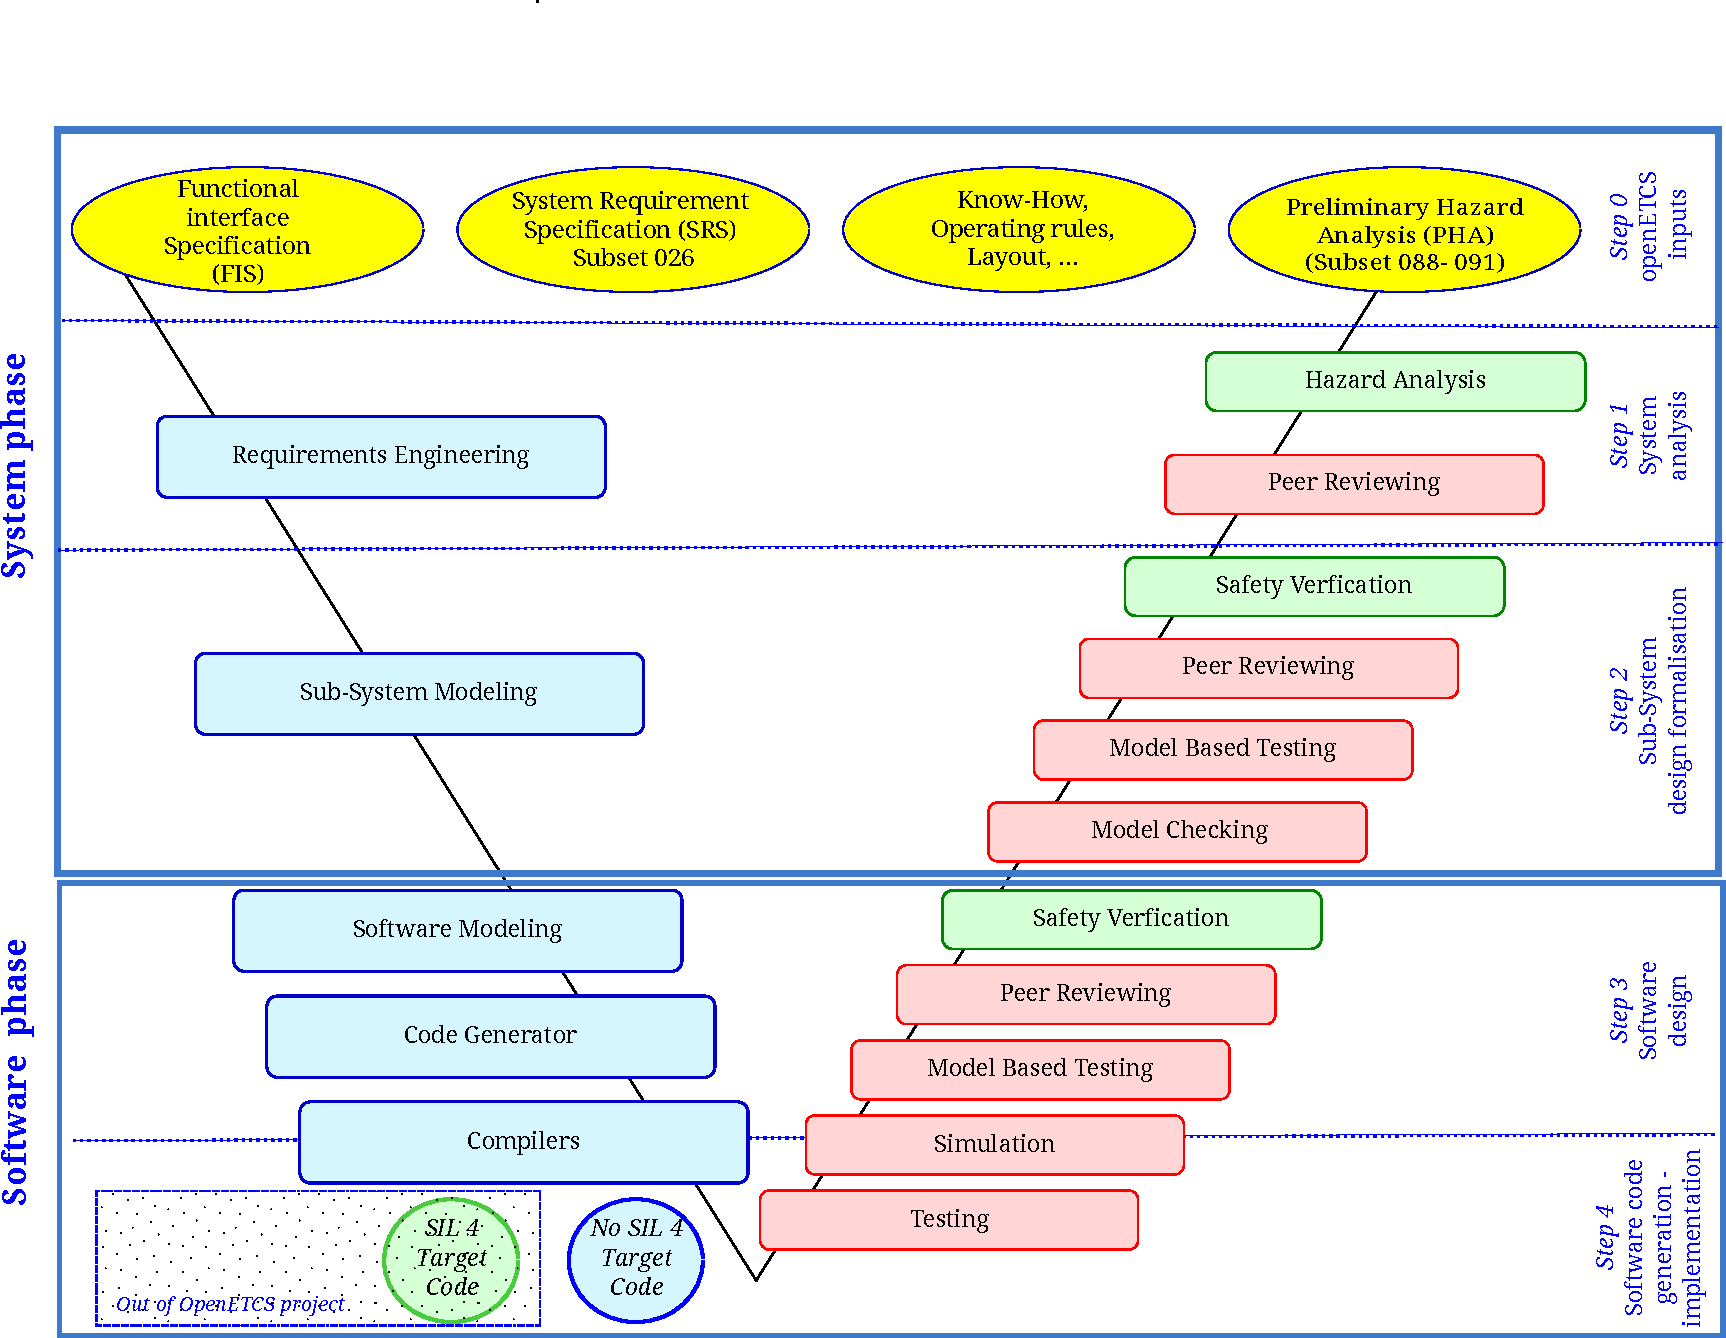
\includegraphics[width=\textwidth]{images/WholeProcess_Activities}
  \caption{openETCS Process Tool chain activities}
  \label{fig:openETCSActivities}
\end{figure}

\todo[inline]{add description of each activities}

%----------------------------------------------------
\section{Management tools}
%----------------------------------------------------
\todo[inline] {add the list of the management tools and a description}
\begin{itemize}
\item Version Management\\
Version management of the artifacts and the openETCS glue code 
\item Tool version Management \\
Keep track of the compatible and status version of each tools. 
\item Collaborative work
\item Project  Management
\item Build system
\item Non regression test
\item Configuration Manger to manage modification and change in tools
\end{itemize}



%%% Local Variables: 
%%% mode: latex
%%% TeX-master: "WP7-Toolchain_architecture"
%%% End: 
